\documentclass{beamer}
\usepackage[francais,english]{babel}
\usepackage[T1]{fontenc}
\usepackage{amsmath,amsfonts,amssymb}
\usepackage{xspace}

\mode<presentation> {\usetheme{CambridgeUS}}
\usecolortheme{spruce}
%%dolphin, spruce

\usepackage{graphicx} % Allows including images
\usepackage{booktabs} % Allows the use of \toprule, \midrule and \bottomrule in tables


\title{Exp�rimentation du r�seau de neurones U-net pour la d�t�ction de pollutions maritimes}
\author{Herm�n�gilde Valentin}
\institute{ENS Lyon}
%\medskip
\date{\today}

\begin{document}

\begin{frame}
  \titlepage
\end{frame}

\section{Probl�me}

\frame{\tableofcontents[currentsection]}

\begin{frame}
  \frametitle{O� est la pollution?}
  \begin{figure}
    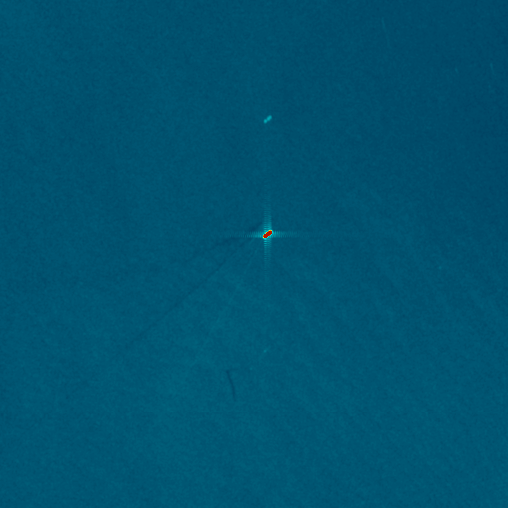
\includegraphics[height=180pt]{images/nrcs_ex.png}
  \end{figure}
\end{frame}

\begin{frame}
  \frametitle{O� est la pollution?}
  \begin{figure}
    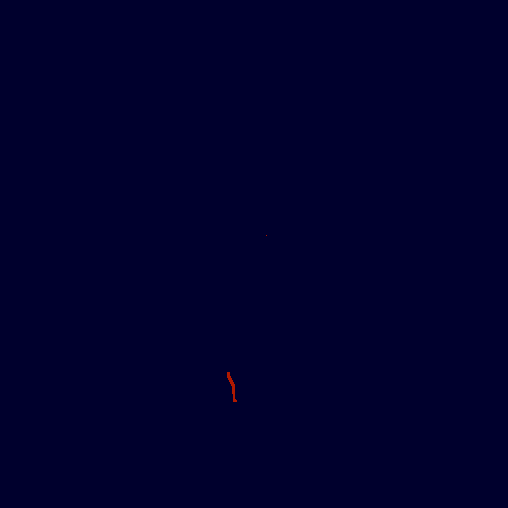
\includegraphics[height=180pt]{images/mask_ex.png}
  \end{figure}
\end{frame}

\begin{frame}
  \frametitle{Et maintenant?}
  \begin{figure}
    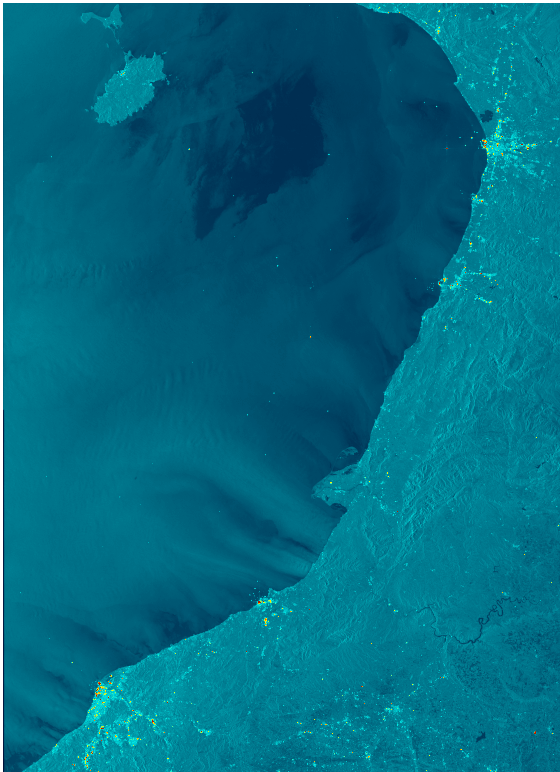
\includegraphics[height=180pt]{images/nrcs_full.png}
  \end{figure}
\end{frame}

\begin{frame}
  \frametitle{Et l�?}
  \begin{figure}
    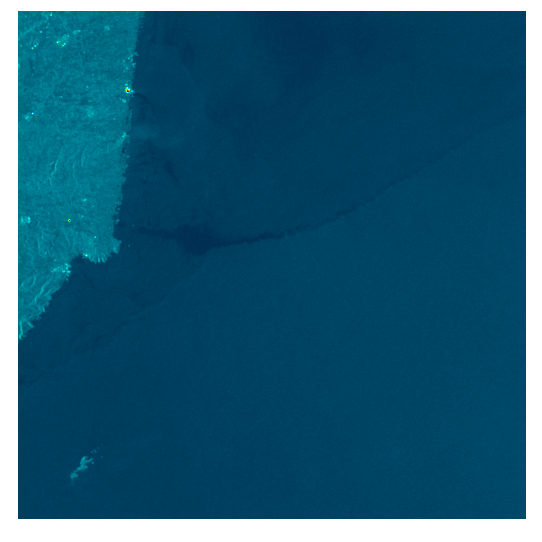
\includegraphics[height=180pt]{images/piege.png}
  \end{figure}
\end{frame}

\section{U-net}

\frame{\tableofcontents[currentsection]}

\begin{frame}
  \frametitle{U-net}
  \begin{figure}
    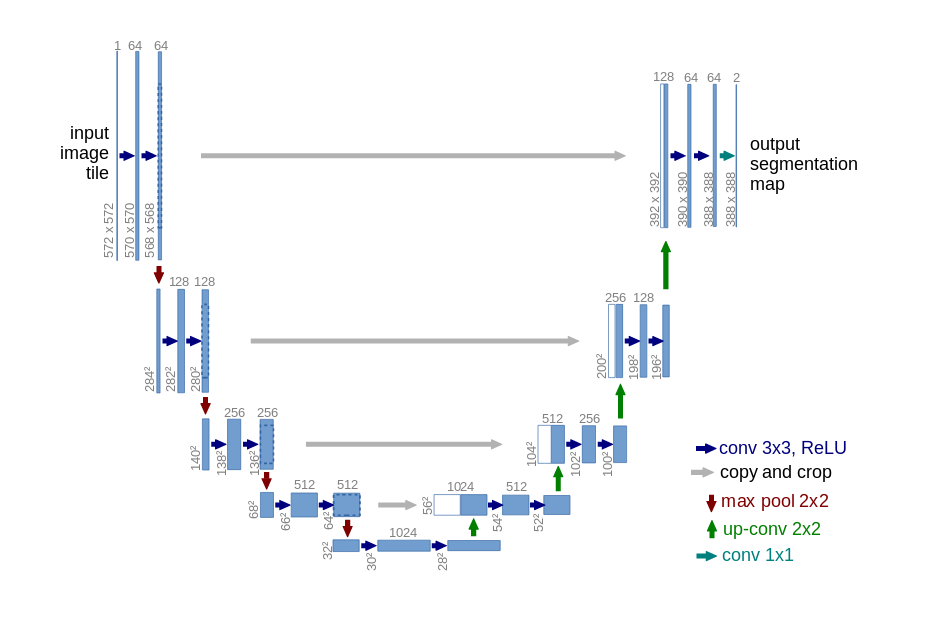
\includegraphics[height=200pt]{images/unet_orig.png}
  \end{figure}
\end{frame}

\begin{frame}
  \frametitle{Inter�ts d'U-net}
  \begin{itemize}
  \item Analyse � diff�rentes �chelles \pause
  \item Bonne localisation \pause
  \item Entra�nable sur des petits jeux de donn�es (selon le papier)
  \end{itemize}
\end{frame}

\section{D�boires et r�sultats}

\frame{\tableofcontents[currentsection]}

\begin{frame}
  R�seau de base: 98\% de pr�cision sur la segmentation... \pause \\
  Sur 98\% de mer \\ \pause
  \medskip
  Avec des poids sur les pollutions: un peu mieux (un petit tiers de pollutions detect�es), mais au prix de nombreuses fausses alertes \\ \pause
  On a effectivement une convergence rapide
\end{frame}

\begin{frame}
  \frametitle{R�seaux plus profonds}
  \begin{figure}
    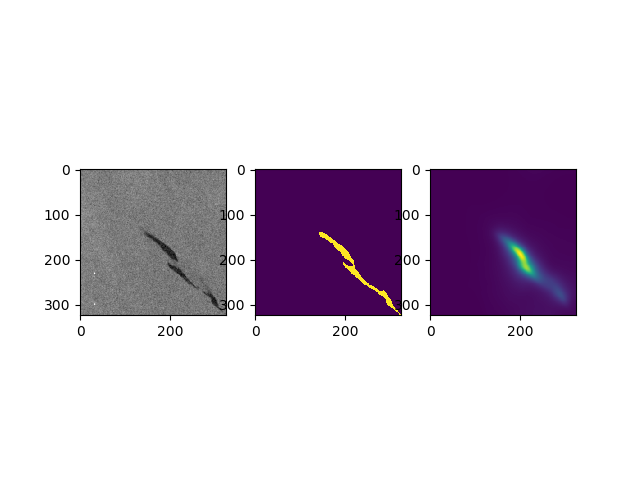
\includegraphics[height=150pt]{images/fake1.png}
    \caption{Sans �chelle...}
  \end{figure}
\end{frame}

\begin{frame}
  \frametitle{Probl�mes de fond}
  Fort niveau d'�nergie sur les bateaux (affichage en log)
  \begin{figure}
    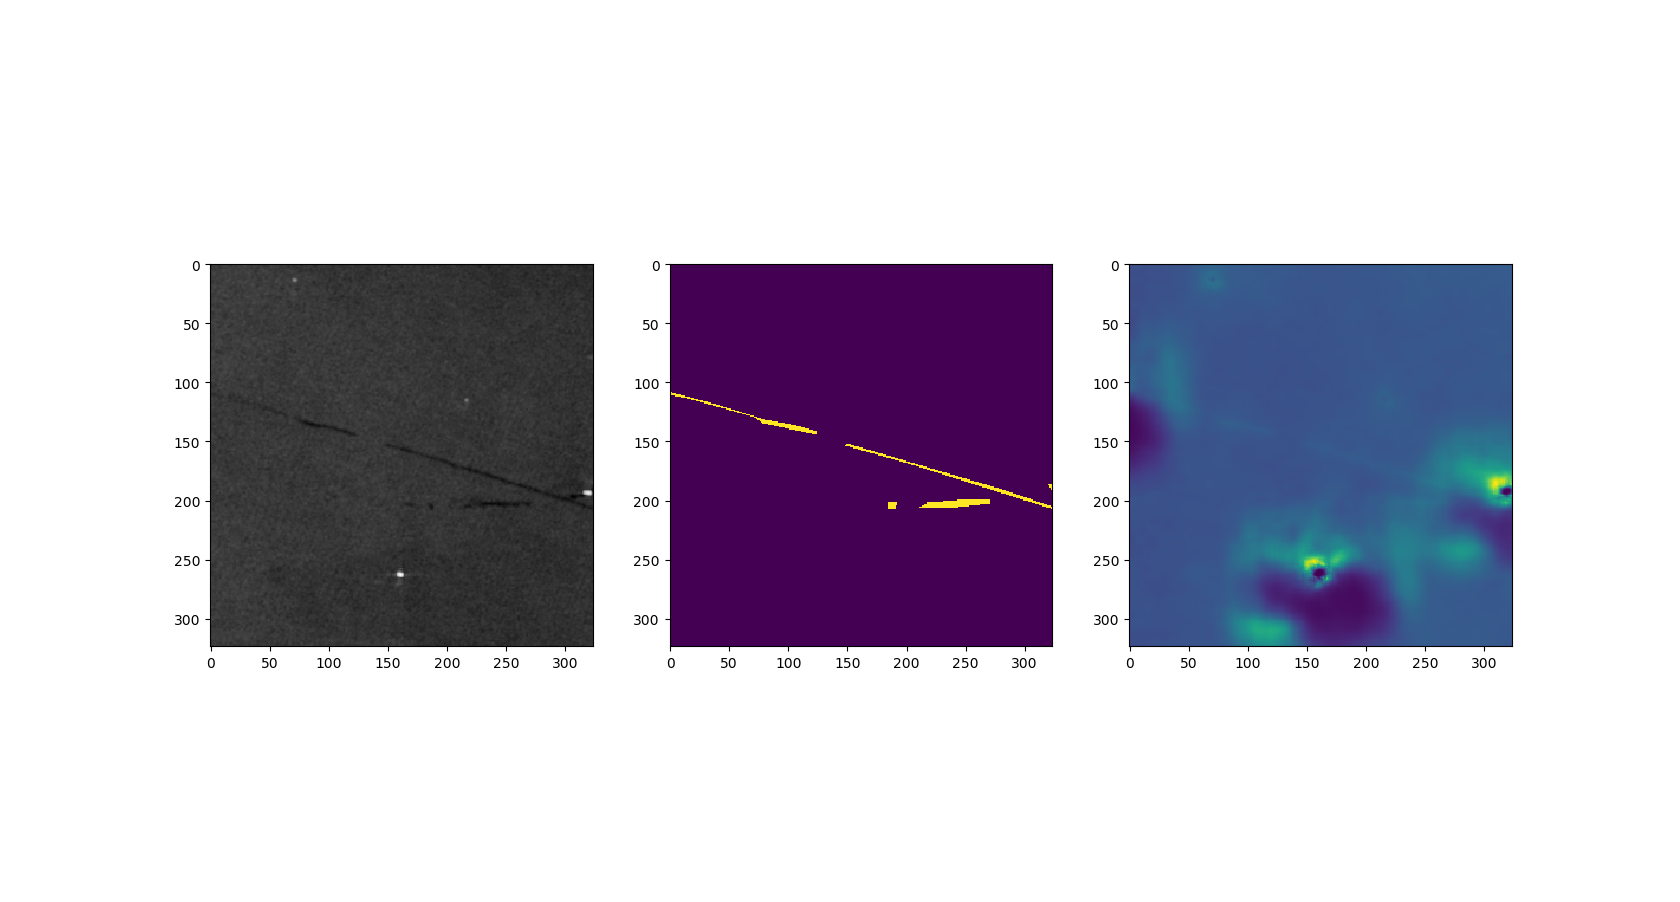
\includegraphics[height=200pt]{images/deep6_2.png}
  \end{figure}
\end{frame}

\begin{frame}
  \frametitle{Probl�mes de fond}
  98\% d'eau, moins de 10 ppm de pollution
  \begin{figure}
    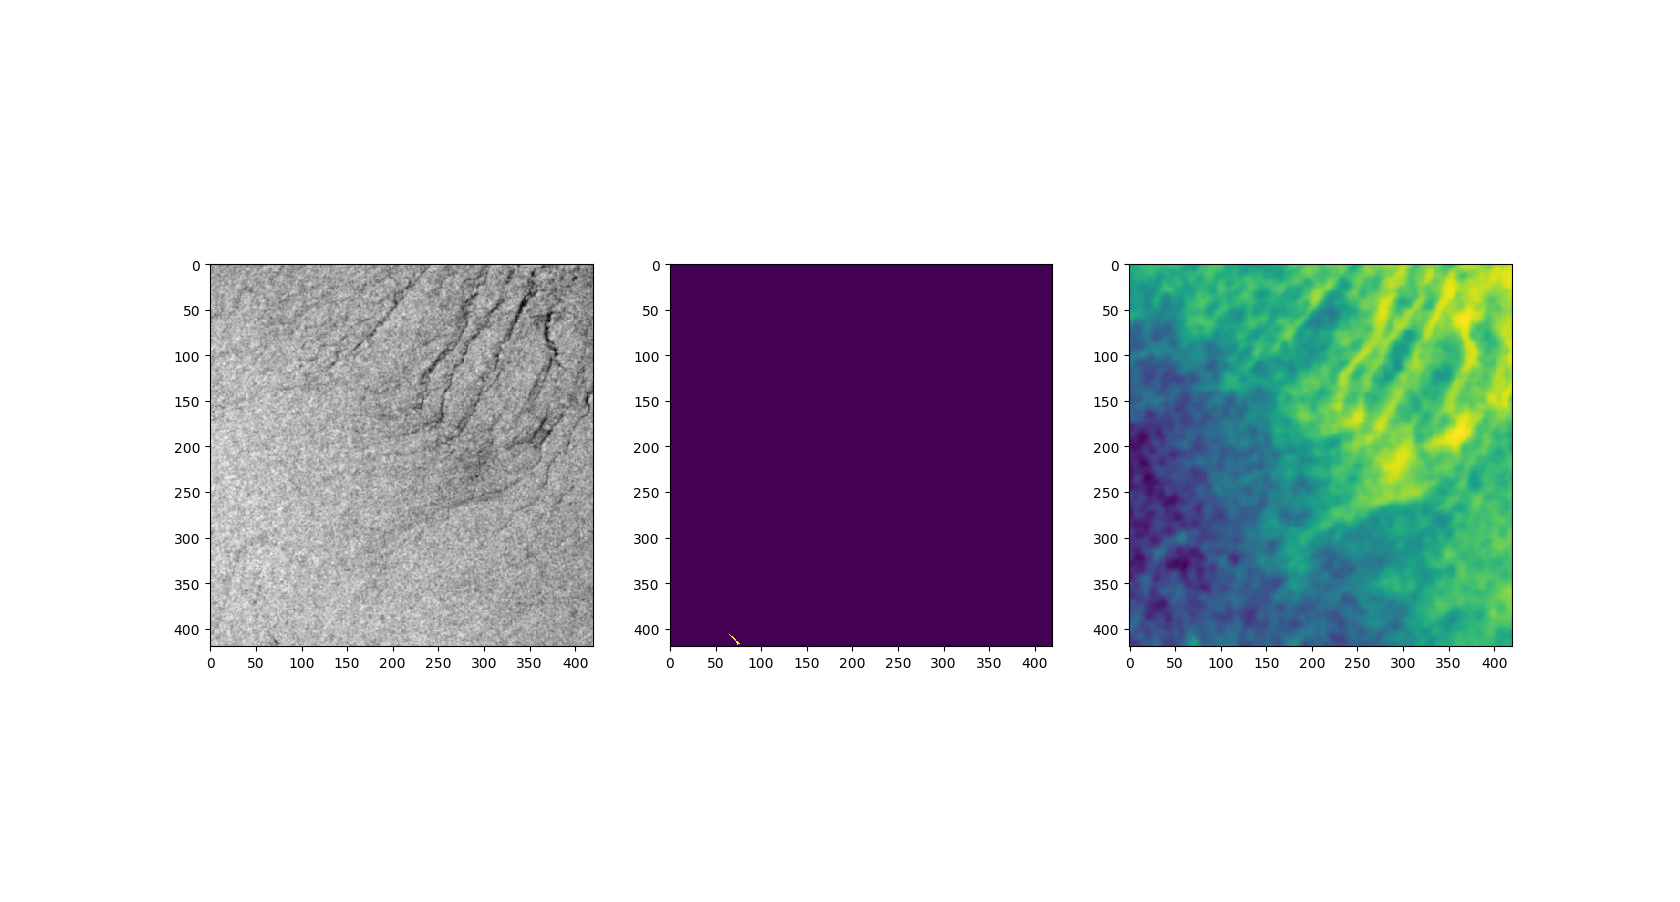
\includegraphics[height=200pt]{images/diff_land1.png}
  \end{figure}
\end{frame}



\begin{frame}
  \frametitle{Solution?}
  \begin{itemize}
  \item Surrepr�senter les pollutions, mais pas trop
  \item Fournir la carte des bateaux en entr�e
  \end{itemize}
  \begin{figure}
    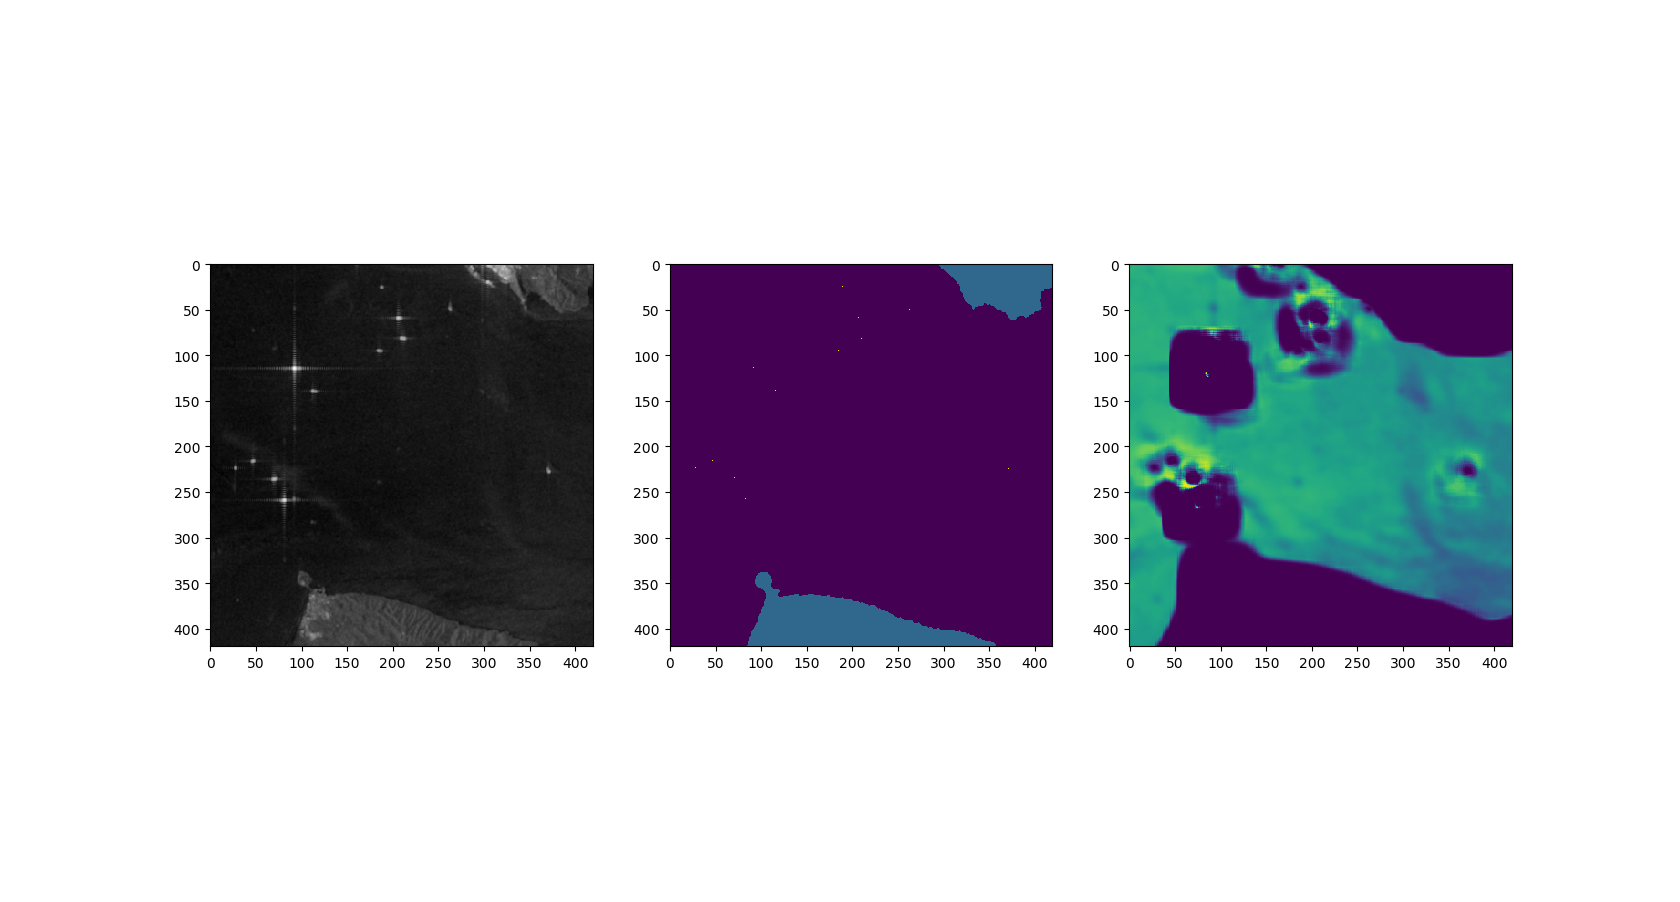
\includegraphics[height=200pt]{images/boat2_land1.png}
  \end{figure}
\end{frame}

\begin{frame}
  \frametitle{Plus de donn�es?}
  Le niveau d'intensit� sur l'image SAR d�pend de la direction et la vitesse du vent, et de l'angle d'incidence (GMF).\pause
  Qui sont fournis.
\end{frame}

\begin{frame}
  \frametitle{Plus de donn�es?}
  \begin{figure}
    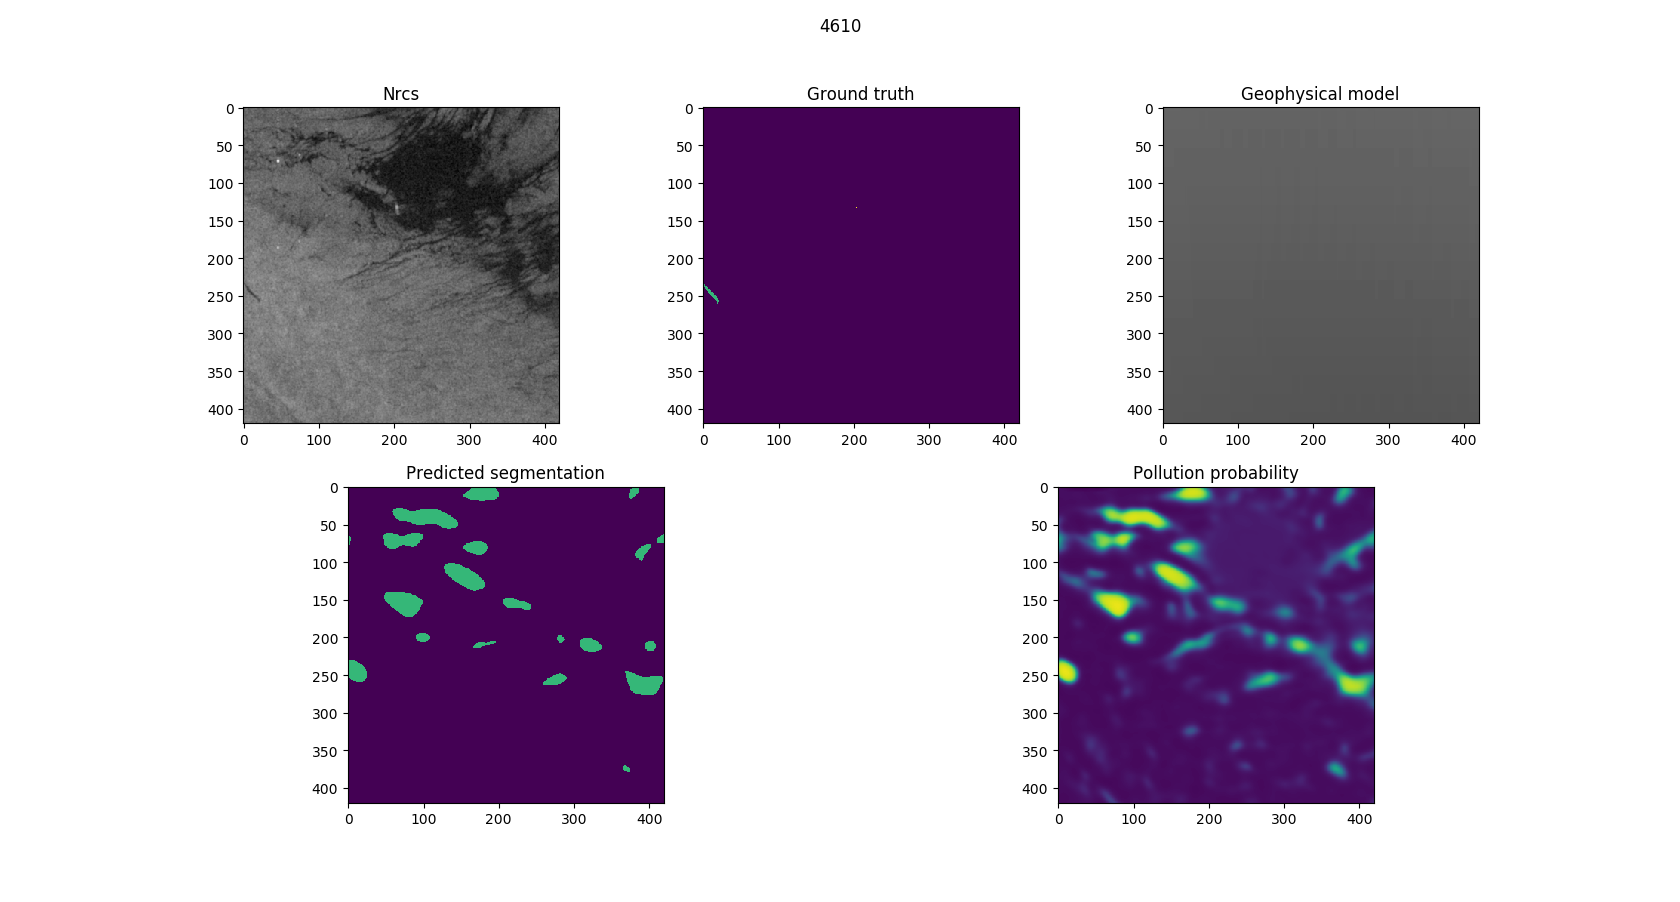
\includegraphics[height=200pt]{images/hard_gmf1.png}
  \end{figure}
\end{frame}

\begin{frame}
  \frametitle{ROC}
  \begin{figure}
    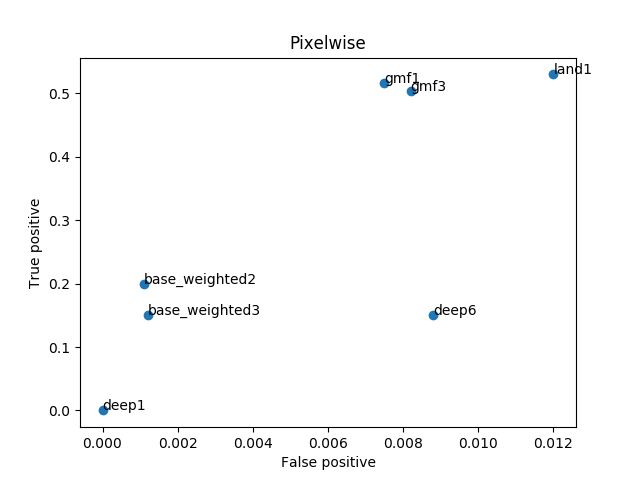
\includegraphics[height=200pt]{images/ROC_pixel.png}
  \end{figure}
\end{frame}

\begin{frame}
  \frametitle{ROC}
  \begin{figure}
    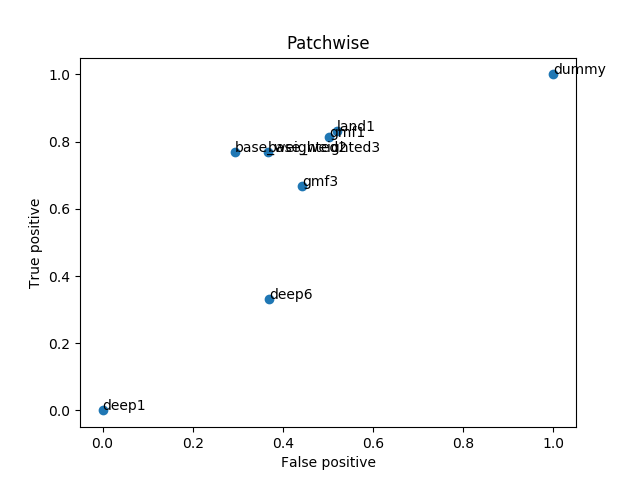
\includegraphics[height=200pt]{images/ROC_patch.png}
  \end{figure}
\end{frame}

\section{A faire (si je n'avais pas eu que six semaines)}

\frame{\tableofcontents[currentsection]}

\begin{frame}
  \frametitle{Comprendre mes r�seaux}
  \begin{figure}
    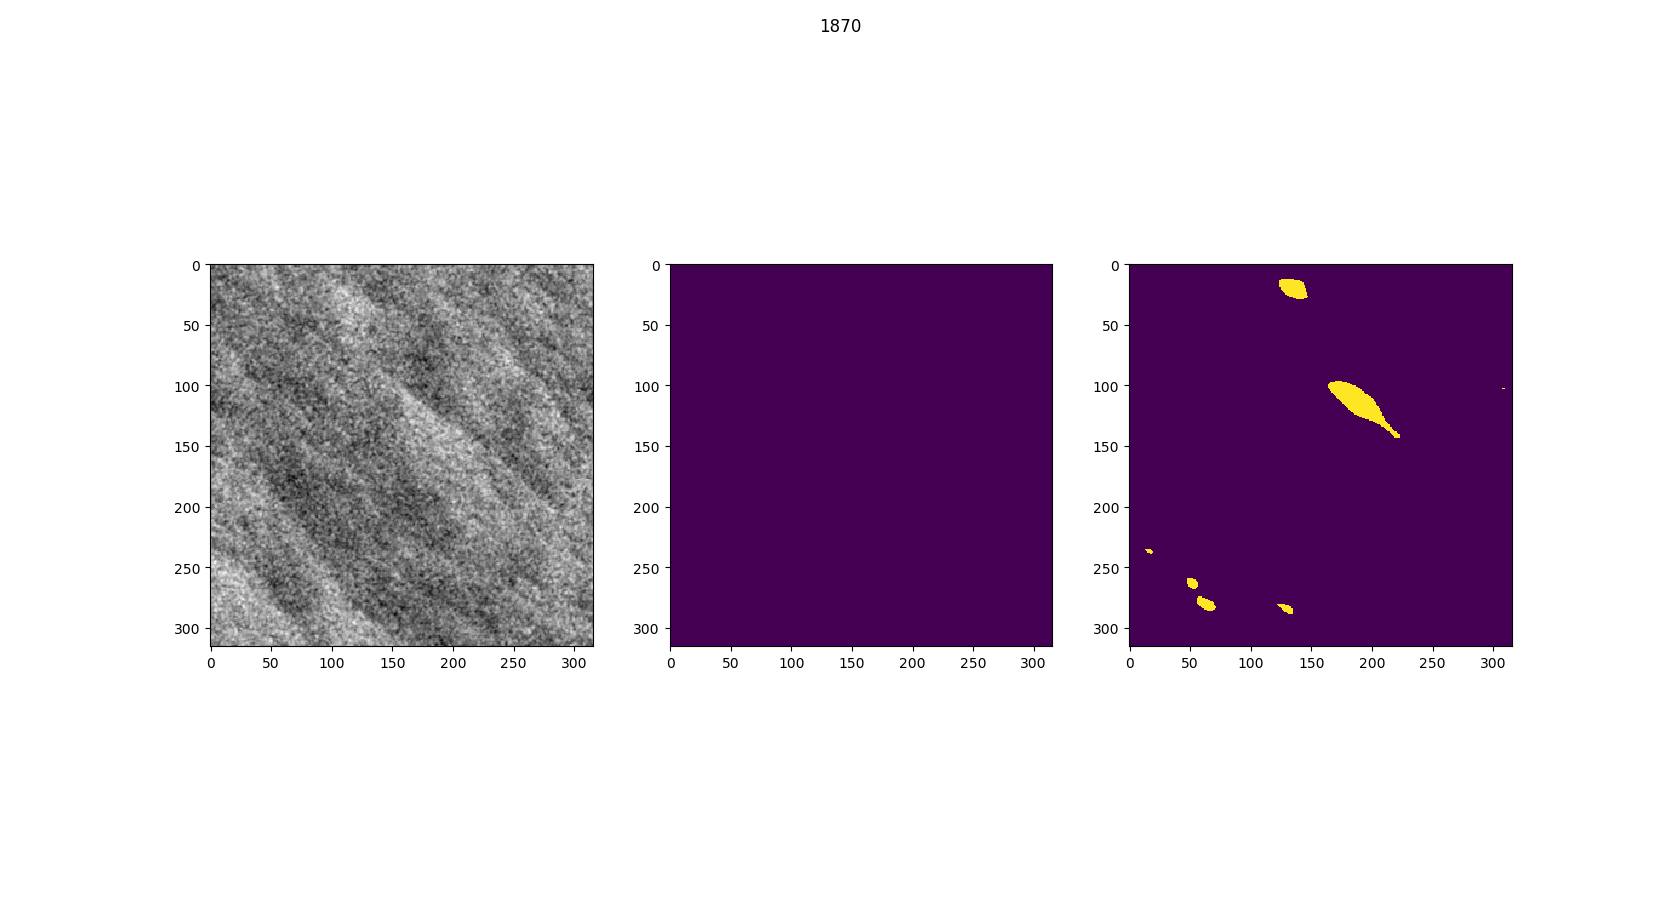
\includegraphics[height=200pt]{images/bad2_gmf3.png}
  \end{figure}
\end{frame}

\begin{frame}
  \frametitle{Comprendre mes r�seaux}
  \begin{figure}
    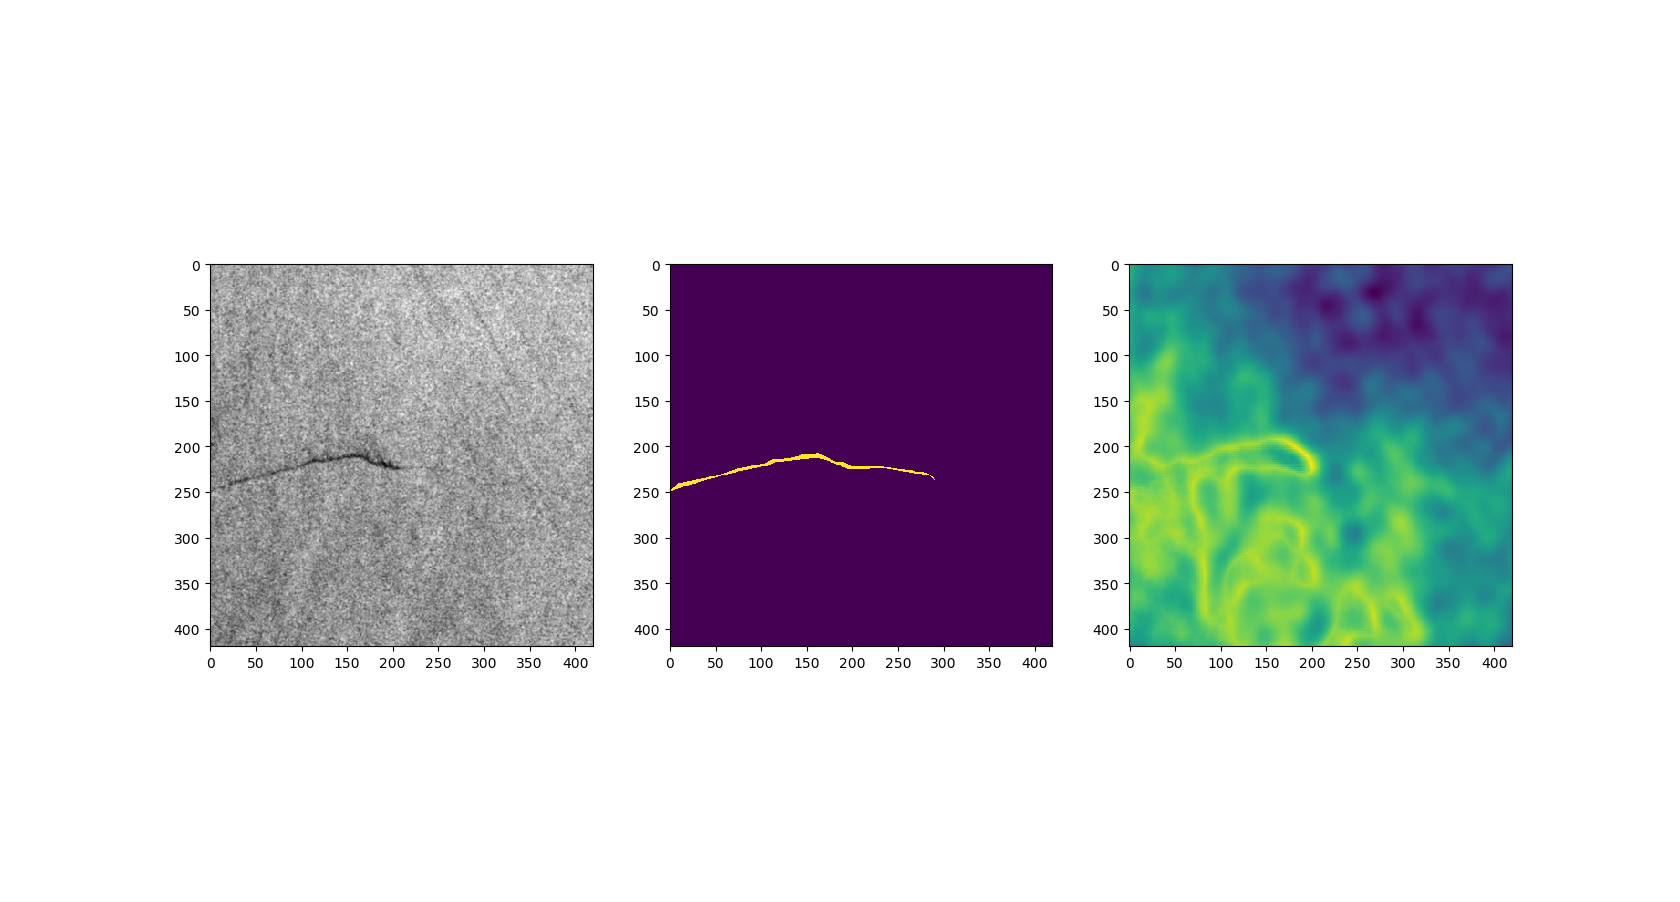
\includegraphics[height=200pt]{images/weird_land1.png}
  \end{figure}
\end{frame}

\begin{frame}
  \frametitle{Apprendre � les faire converger}
  \begin{itemize}
  \item Grande sensibilit� aux les poids donn�es aux diff�rentes classes
  \item Risque de rester coinc� sur un r�seau qui ne voit que de la mer
  \end{itemize}
\end{frame}

\section{Conclusion}

\frame{\tableofcontents[currentsection]}

\begin{frame}
  \frametitle{Conclusion}
  \begin{itemize}
  \item R�seau pas tout � fait pr�t � �tre utilis� en situation r�elle
  \end{itemize}
\end{frame}

\end{document}
